\subsubsection{Varnish}
\label{soa:tecnologias:varnish}

Varnish es un \eng{proxy} reverso \gls{proto:http}, a veces referenciado como acelerador de HTTP o a \eng{web accelerator}, que almacena archivos y fragmentos de archivos en memoria, lo que reduce el tiempo de respuesta y el ancho de banda de red para las mismas solicitudes.\cite[p.~20]{varnish2016}

El proyecto Varnish fue iniciado por Verdens Gang en el 2005, contó con la gerencia, infraestructura y desarrollos adicionales aportados por la comunidad Noruega de Linux, que más tarde pasó a una empresa independiente, Varnish Software bajo licencia BSD.

Como mencionamos anteriormente, Varnish es un acelerador de aplicaciones web, que se instala delante de cualquier servidor HTTP y se configura para almacenar en la caché del servidor una copia del recurso solicitado. Pensado para mejorar el rendimiento de aplicaciones web con contenidos pesados y APIs altamente consumidas, éste será nuestro caso.

\begin{figure}[H]
  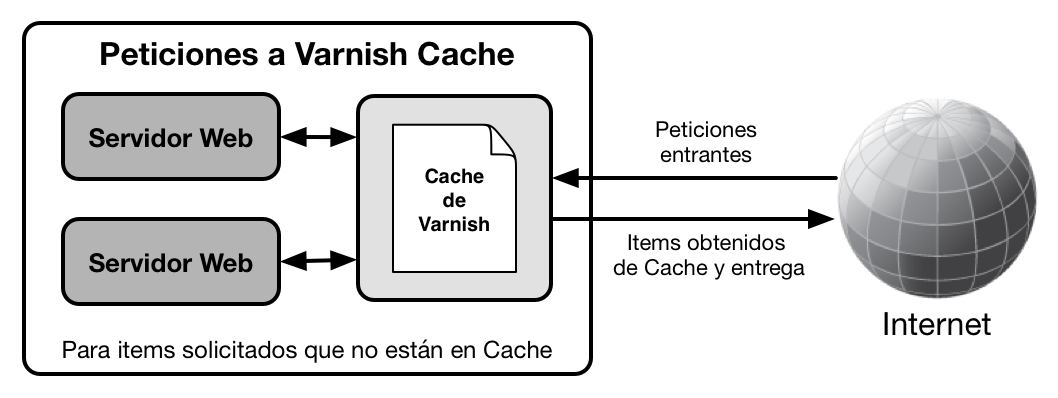
\includegraphics[width=\linewidth]{src/images/03-capitulo-3/tecnologias/varnish/varnish-reverse-proxy.png}
  \caption{Varnish Reverse Proxy}
  \label{fig:varnish}
\end{figure}

\paragraph{Instalación}

Varnish se distribuye en los respositorios de paquetes de Ubuntu, pero puede suceder que el paquete se encuentre desactualizado por lo tanto se recomienda usar los respositorios de paquestes de \url{varnish-cache.org}.

Para usar los respositorios de \url{varnish-cache.org} e instalar Varnish en Ubuntu 14.04, debemos ejecuatar la secuencia de comandos del bloque de código \autoref{soa:tecnologias:varnish-cache:bash-preparacion}:

\begin{listing}[H]
  \bashfile{src/03-capitulo-3/tecnologias/cache/code/varnish/00-preparacion.sh}
  \caption{Instalación de Varnish}
  \label{soa:tecnologias:varnish-cache:bash-preparacion}
\end{listing}
